\section{Opis i~wyniki testowania aplikacji}

Program sprawdzono na cztery sposoby: testami automatycznymi, porównaniem z~przykładami
z~książki, porównaniem wskaźników empirycznych z~teoretycznymi dla prób losowych oraz
podaniem błędnych danych.

\subsection{Testy automatyczne}

Do programu dołączono 64 testy automatyczne, czyli krótkie programy sprawdzające, czy
poszczególne części programu dają oczekiwane wyniki (tab.~\ref{tab:tests}). Uruchamia
się je jednym poleceniem i~wykonują się w~kilka sekund. Wszystkie testy kończą się
powodzeniem.

\begin{table}[H]
  \centering
  \caption{Zakres testów automatycznych}
  \label{tab:tests}
  \small
  \begin{tabular}{@{}>{\raggedright\arraybackslash}p{0.23\textwidth}c>{\raggedright\arraybackslash}p{0.62\textwidth}@{}}
    \toprule
    Część programu & Liczba & Co jest sprawdzane \\
    \midrule
    wyznaczanie wskaźników & 16 & zgodność z~przykładami 5.1--5.4, przedziały o~różnej
      długości, próba niepełna, odrzucanie błędnych danych, grupowanie czasów (w~tym czas
      na granicy przedziału), automatyczny dobór $\Delta t$ \\
    rozkłady trwałości & 8 & odrzucanie niedodatnich parametrów, zbieżność średniej
      z~próby do $ET$, monotoniczność dystrybuant, stała intensywność rozkładu
      wykładniczego \\
    losowanie próby & 6 & powtarzalność próby dla tego samego ziarna, zbieżność $F^*$
      do $F$ oraz $E^*T$ do $ET$ dla $n = 50\,000$ \\
    wczytywanie danych & 6 & separatory, puste wiersze, błędne wiersze i~numer wiersza
      w~komunikacie \\
    zapis liczb & 7 & przecinek i~kropka dziesiętna, błędne liczby, zapis wyników \\
    wykresy & 6 & rysowanie wszystkich wykresów, pominięcie nieokreślonej $\lambda^*$,
      podziałka osi \\
    zapis plików & 3 & format pliku CSV, zapis pliku PNG \\
    okno programu & 12 & obliczenia uruchamiane przyciskiem z~każdego formularza, treść
      komunikatów o~błędach, zapis wyników i~wykresów \\
    \bottomrule
  \end{tabular}
\end{table}

Testy okna programu uruchamiają je w~trybie testowym, wypełniają formularze
i~,,naciskają'' przyciski, a~następnie sprawdzają wyświetlone wyniki. Zrzuty okna
zamieszczone w~tym sprawozdaniu zostały zapisane podczas tych testów.


\subsection{Zgodność z~przykładami z~książki}

Dane z~przykładu 5.1 w~\cite{prazewska}: próbka $n(0) = 35$ kondensatorów
elektrolitycznych, badanie do uszkodzenia ostatniego elementu, rejestracja co godzinę;
liczby uszkodzeń w~kolejnych godzinach: 0, 3, 3, 5, 8, 7, 6, 2, 1, 0. Dane te są
wczytywane w~zakładce ,,Tabela uszkodzeń'' po uruchomieniu programu
(rys.~\ref{fig:book-results} i~\ref{fig:book-charts}). W~tab.~\ref{tab:book-fr}
i~\ref{tab:book-fl} zestawiono wyniki programu z~tablicami z~przykładów 5.1--5.4.

\begin{table}[H]
  \centering
  \caption{Dystrybuanta i~funkcja niezawodności: program i~książka (przykłady 5.1 i~5.2)}
  \label{tab:book-fr}
  \small
  \begin{tabular}{@{}cc@{\qquad}cc@{\qquad}cc@{}}
    \toprule
    & & \multicolumn{2}{c@{\qquad}}{$F^*(t_i)$} & \multicolumn{2}{c}{$R^*(t_i)$} \\
    $t_i$ [h] & $m(t_i)$ & program & książka & program & książka \\
    \midrule
    1 & 0 & 0,0000 & 0 & 1,0000 & 1 \\
    2 & 3 & 0,0857 & 0,086 & 0,9143 & 0,914 \\
    3 & 3 & 0,1714 & 0,171 & 0,8286 & 0,828 \\
    4 & 5 & 0,3143 & 0,314 & 0,6857 & 0,686 \\
    5 & 8 & 0,5429 & 0,543 & 0,4571 & 0,457 \\
    6 & 7 & 0,7429 & 0,743 & 0,2571 & 0,257 \\
    7 & 6 & 0,9143 & 0,914 & 0,0857 & 0,086 \\
    8 & 2 & 0,9714 & 0,971 & 0,0286 & 0,029 \\
    9 & 1 & 1,0000 & 1 & 0,0000 & 0 \\
    10 & 0 & 1,0000 & 1 & 0,0000 & 0 \\
    \bottomrule
  \end{tabular}
\end{table}

\begin{table}[H]
  \centering
  \caption{Gęstość i~intensywność uszkodzeń: program i~książka (przykłady 5.3 i~5.4)}
  \label{tab:book-fl}
  \small
  \begin{tabular}{@{}c@{\qquad}cc@{\qquad}cc@{}}
    \toprule
    & \multicolumn{2}{c@{\qquad}}{$f^*(t_i)$ [1/h]} & \multicolumn{2}{c}{$\lambda^*(t_i)$ [1/h]} \\
    $t_i$ [h] & program & książka & program & książka \\
    \midrule
    1 & 0,00000 & 0 & 0,00000 & 0 \\
    2 & 0,08571 & 0,086 & 0,08571 & 0,086 \\
    3 & 0,08571 & 0,086 & 0,09375 & 0,095 \\
    4 & 0,14286 & 0,143 & 0,17241 & 0,172 \\
    5 & 0,22857 & 0,228 & 0,33333 & 0,333 \\
    6 & 0,20000 & 0,2 & 0,43750 & 0,437 \\
    7 & 0,17143 & 0,171 & 0,66667 & 0,667 \\
    8 & 0,05714 & 0,057 & 0,66667 & 0,667 \\
    9 & 0,02857 & 0,0286 & 1,00000 & 1,0 \\
    10 & 0,00000 & --- & --- & --- \\
    \bottomrule
  \end{tabular}
\end{table}

Wyniki programu zgadzają się z~książką. Największa różnica wynosi $0{,}00125$
i~dotyczy $\lambda^*(t_3) = 3/32 = 0{,}09375$, dla której w~książce podano $0{,}095$.
Pozostałe różnice są na trzecim miejscu po przecinku i~wynikają z~obcinania cyfr
w~książce, np. $R^*(t_3) = 29/35 = 0{,}82857$ (w~książce $0{,}828$) oraz
$f^*(t_5) = 8/35 = 0{,}22857$ (w~książce $0{,}228$). Dla $t_{10}$ książka nie podaje
$f^*$ ani $\lambda^*$; program wyznacza $f^*(t_{10}) = 0$, a~$\lambda^*(t_{10})$
oznacza jako nieokreśloną, ponieważ po dziewiątej godzinie nie ma już elementów
zdatnych.

Dla tych danych program podaje $E^*T = 5{,}2571$~h ze wzoru (5-15), przyjmując za
trwałość chwilę rejestracji uszkodzenia ($184/35$), oraz $E^*T = 4{,}7571$~h
z~całkowania $R^*(t)$. Różnica wynosi dokładnie $0{,}5$~h, czyli połowę odstępu między
rejestracjami: pierwsza wartość zakłada, że elementy uszkadzały się na końcu każdej
godziny, a~druga -- że równomiernie w~jej trakcie. Poprawność obu wartości sprawdzono
rachunkiem ręcznym.

\begin{figure}[H]
  \centering
  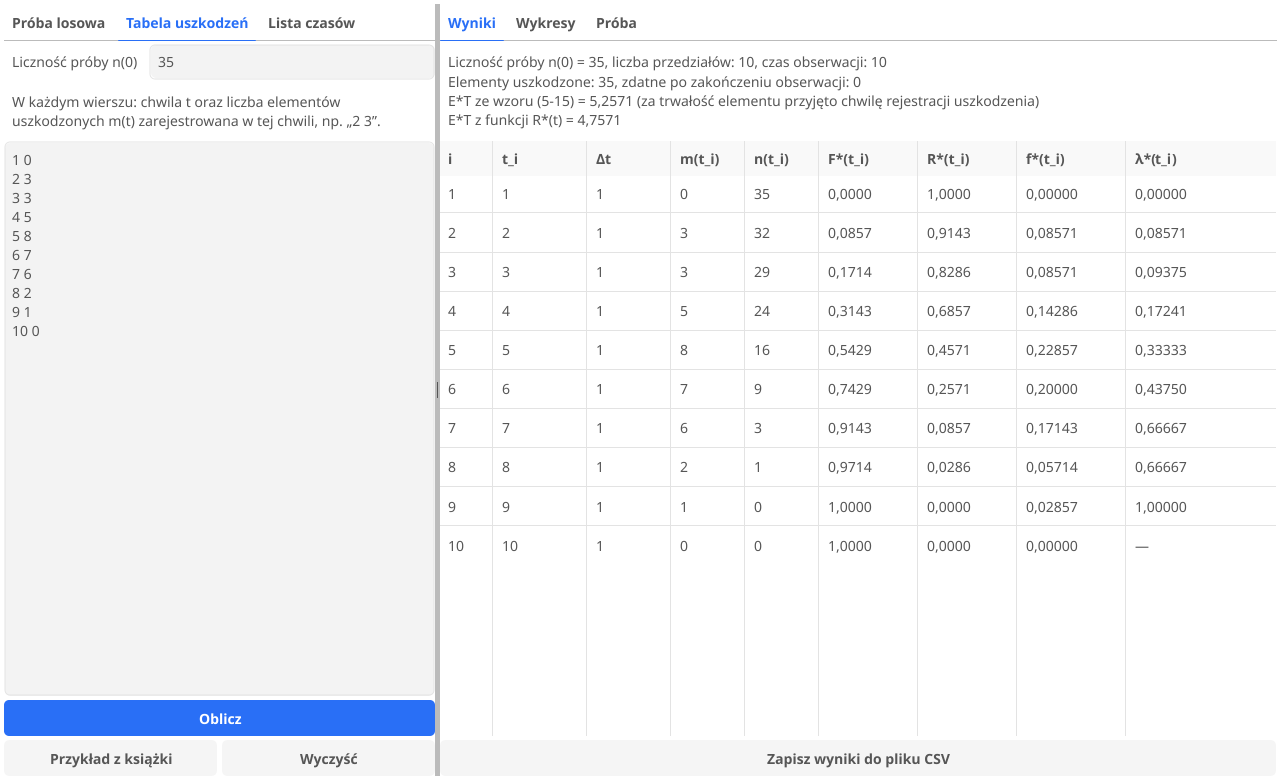
\includegraphics[width=\textwidth]{02_table_results}
  \caption{Wyniki programu dla danych z~przykładu 5.1}
  \label{fig:book-results}
\end{figure}

\begin{figure}[H]
  \centering
  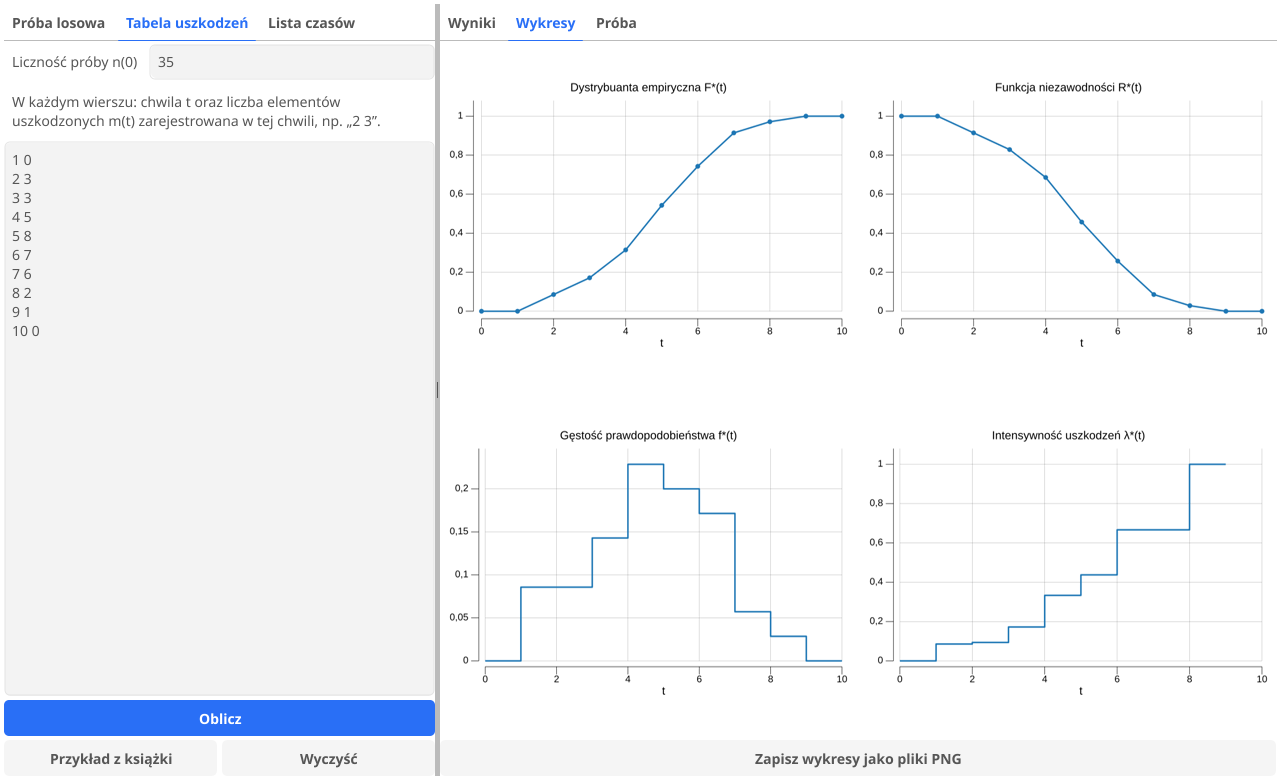
\includegraphics[width=\textwidth]{03_table_charts}
  \caption{Wykresy wskaźników dla danych z~przykładu 5.1}
  \label{fig:book-charts}
\end{figure}

\subsection{Próba losowa a~rozkład teoretyczny}

Dla każdego z~trzech rozkładów wylosowano próby o~liczności 100, 1000 i~10\,000
(ziarno generatora~1, parametry domyślne, $\Delta t$ dobierane automatycznie)
i~porównano wskaźniki empiryczne z~teoretycznymi (tab.~\ref{tab:random}). Wyniki można
odtworzyć w~programie, wpisując te same ustawienia.

\begin{table}[H]
  \centering
  \caption{Wskaźniki empiryczne dla prób losowych; $\max|F^* - F|$ to największa różnica
    między dystrybuantą empiryczną i~teoretyczną w~chwilach $t_i$}
  \label{tab:random}
  \small
  \begin{tabular}{@{}lrrrrrrr@{}}
    \toprule
    Rozkład & $n$ & $\Delta t$ & $k$ & $E^*T$ (5-15) & $E^*T$ z~$R^*$ & $ET$ & $\max|F^* - F|$ \\
    \midrule
    wykładniczy & 100 & 50 & 10 & 104,82 & 103,50 & 100,00 & 0,0479 \\
    $\lambda = 0{,}01$ & 1000 & 25 & 27 & 100,57 & 101,08 & 100,00 & 0,0099 \\
    & 10\,000 & 20 & 47 & 99,00 & 99,30 & 100,00 & 0,0043 \\
    \midrule
    Weibulla & 100 & 25 & 9 & 90,94 & 89,00 & 88,62 & 0,0479 \\
    $\beta = 2$, $\eta = 100$ & 1000 & 10 & 26 & 88,93 & 88,67 & 88,62 & 0,0099 \\
    & 10\,000 & 10 & 31 & 88,26 & 88,22 & 88,62 & 0,0049 \\
    \midrule
    normalny & 100 & 20 & 7 & 101,30 & 100,40 & 100,00 & 0,0513 \\
    $\mu = 100$, $\sigma = 20$ & 1000 & 10 & 17 & 100,23 & 100,22 & 100,00 & 0,0125 \\
    & 10\,000 & 5 & 37 & 99,71 & 99,73 & 100,00 & 0,0074 \\
    \bottomrule
  \end{tabular}
\end{table}

Wraz ze wzrostem liczności próby wskaźniki empiryczne zbliżają się do teoretycznych:
największa różnica dystrybuant maleje z~około $0{,}05$ dla $n = 100$ do poniżej
$0{,}01$ dla $n = 10\,000$, a~błąd względny $E^*T$ -- z~kilku procent do najwyżej
jednego procenta. Wykresy (rys.~\ref{fig:exponential}--\ref{fig:normal}) pokazują
zgodność przebiegów empirycznych (linia ciągła) z~teoretycznymi (linia przerywana).
Kształt $\lambda^*(t)$ odpowiada teorii: intensywność jest stała dla rozkładu
wykładniczego i~rośnie dla rozkładów Weibulla ($\beta = 2$) i~normalnego. Na końcu
osi czasu przebieg $\lambda^*$ staje się nieregularny, ponieważ zostaje już tylko
kilka zdatnych elementów i~pojedyncze uszkodzenie silnie zmienia wynik.

\begin{figure}[H]
  \centering
  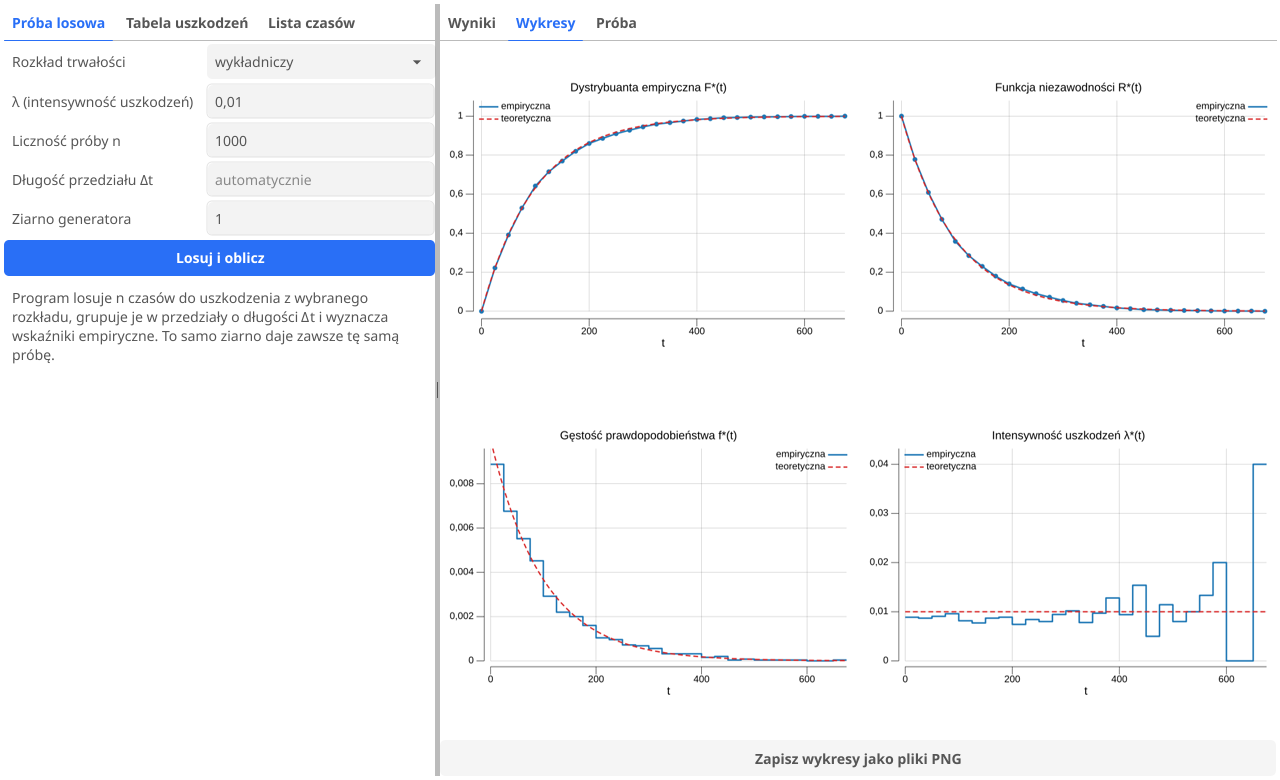
\includegraphics[width=\textwidth]{07_random_exponential_charts}
  \caption{Próba losowa z~rozkładu wykładniczego, $n = 1000$, ziarno 1}
  \label{fig:exponential}
\end{figure}

\begin{figure}[H]
  \centering
  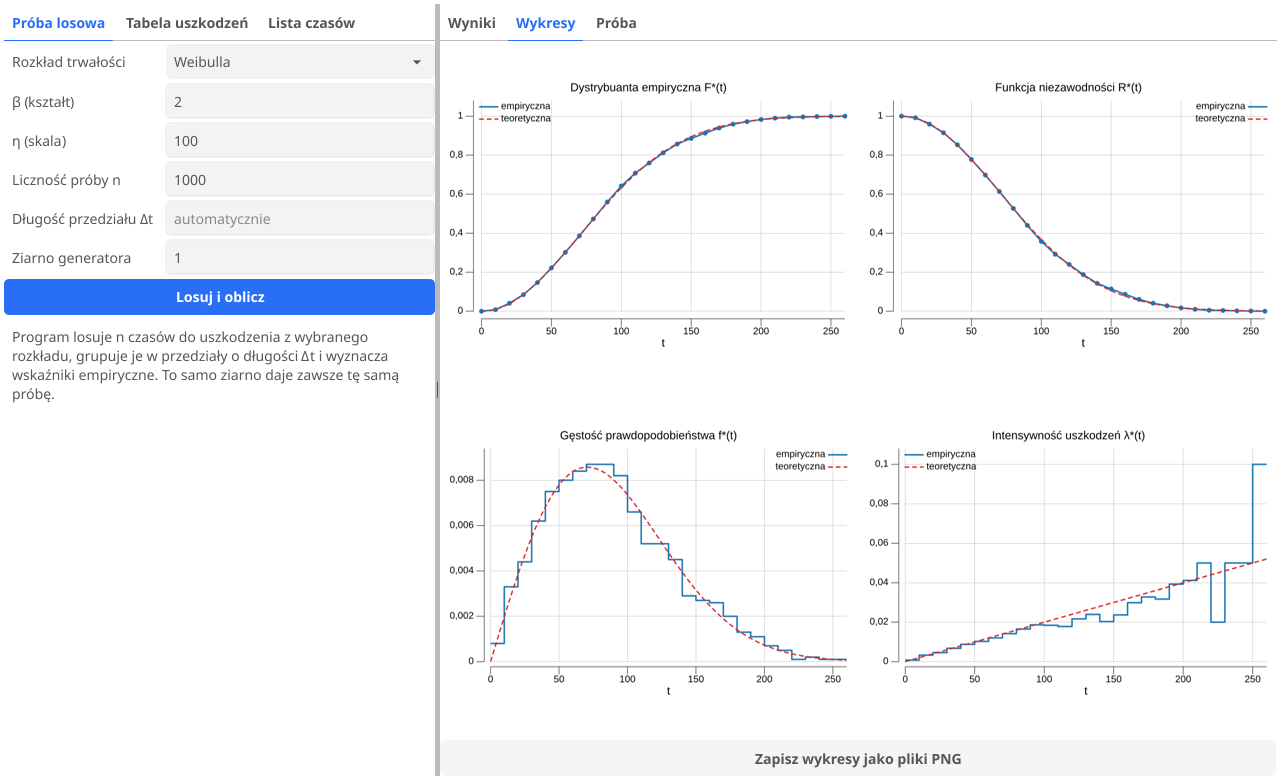
\includegraphics[width=\textwidth]{07_random_weibull_charts}
  \caption{Próba losowa z~rozkładu Weibulla, $n = 1000$, ziarno 1}
  \label{fig:weibull}
\end{figure}

\begin{figure}[H]
  \centering
  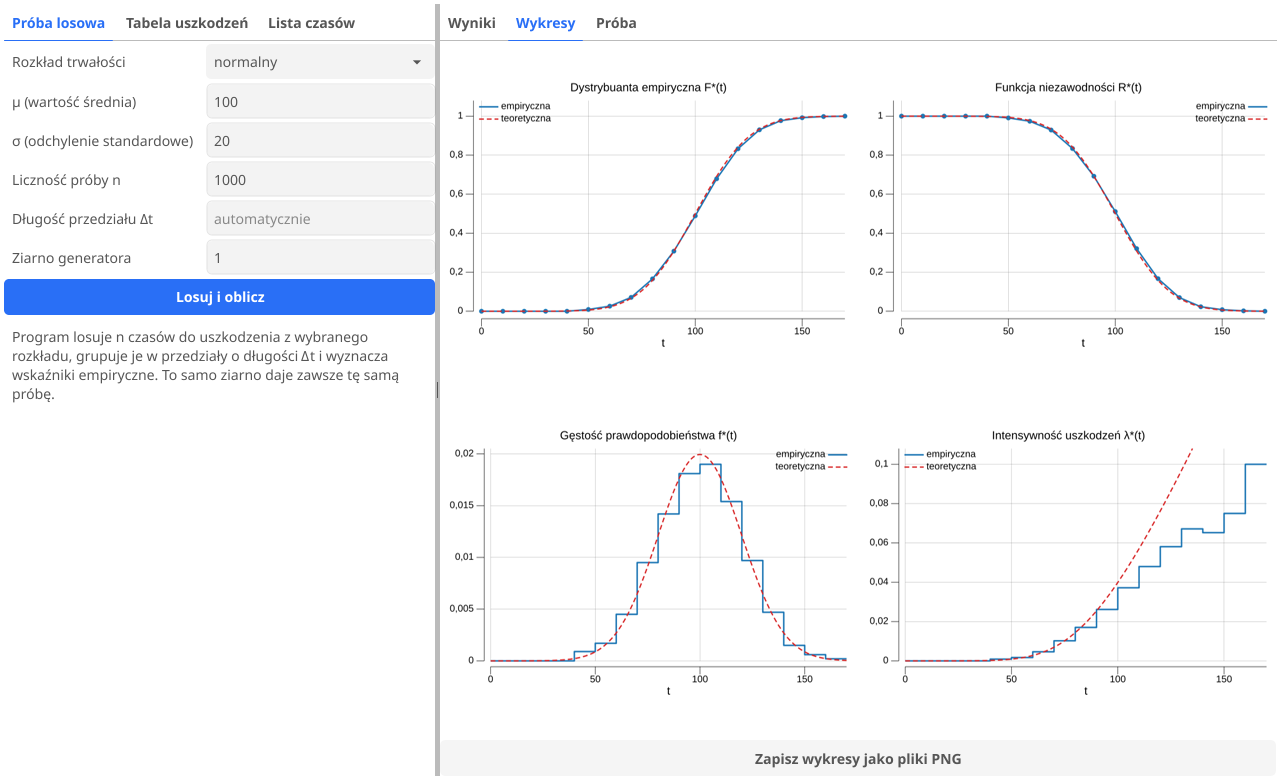
\includegraphics[width=\textwidth]{07_random_normal_charts}
  \caption{Próba losowa z~rozkładu normalnego, $n = 1000$, ziarno 1}
  \label{fig:normal}
\end{figure}

\subsection{Wpływ długości przedziału na wyniki}

Na rys.~\ref{fig:exponential} empiryczna intensywność uszkodzeń leży nieco poniżej
teoretycznej. Nie jest to błąd programu, lecz cecha wzoru (5-12): odnosi on
uszkodzenia z~całego przedziału do liczby elementów zdatnych na jego początku,
podczas gdy w~trakcie przedziału elementów zdatnych ubywa. Dla rozkładu wykładniczego
udział elementów uszkodzonych w~przedziale wynosi średnio $1 - e^{-\lambda \Delta t}$,
więc wzór (5-12) daje przeciętnie
\begin{equation*}
  \lambda^* \approx \frac{1 - e^{-\lambda \Delta t}}{\Delta t} < \lambda.
\end{equation*}
Sprawdzono to dla próby z~rozkładu wykładniczego ($\lambda = 0{,}01$, $n = 10\,000$,
ziarno~1), zmieniając tylko długość przedziału (tab.~\ref{tab:step}).

\begin{table}[H]
  \centering
  \caption{Wpływ długości przedziału $\Delta t$ na wyniki; rozkład wykładniczy,
    $\lambda = 0{,}01$, $ET = 100$}
  \label{tab:step}
  \small
  \begin{tabular}{@{}rccccc@{}}
    \toprule
    $\Delta t$ & $\lambda^*(t_1)$ & $\lambda^*(t_2)$ & $\lambda^*(t_3)$
      & $\dfrac{1 - e^{-\lambda\Delta t}}{\Delta t}$ & $E^*T$ z~$R^*$ \\
    \midrule
    100 & 0,00635 & 0,00636 & 0,00640 & 0,00632 & 107,15 \\
    50 & 0,00795 & 0,00787 & 0,00788 & 0,00787 & 101,01 \\
    25 & 0,00885 & 0,00906 & 0,00880 & 0,00885 & 99,50 \\
    10 & 0,00942 & 0,00966 & 0,00951 & 0,00952 & 99,09 \\
    5 & 0,00984 & 0,00947 & 0,00991 & 0,00975 & 99,00 \\
    \bottomrule
  \end{tabular}
\end{table}

Wartości wyznaczone przez program zgadzają się z~przewidywanymi. Dla $\Delta t = 100$
intensywność jest zaniżona o~blisko 37\%, a~dla $\Delta t = 5$ -- o~około 2,5\%.
Podobnie zachowuje się $E^*T$ wyznaczana z~$R^*(t)$: przy grubych przedziałach metoda
trapezów zawyża pole pod wypukłą krzywą, a~wraz ze zmniejszaniem $\Delta t$ wynik
zbliża się do wartości $98{,}9976$ otrzymanej ze wzoru (5-15), która od $\Delta t$
nie zależy. Przedział nie może być jednak dowolnie krótki: gdy w~przedziale jest
niewiele uszkodzeń, wartości $f^*$ i~$\lambda^*$ stają się przypadkowe. Dlatego
program domyślnie dobiera około $\sqrt{n}$ przedziałów.

\subsection{Próba niepełna}

Sprawdzono przypadek, w~którym badanie zakończono przed uszkodzeniem wszystkich
elementów. W~zakładce ,,Lista czasów'' podano $n(0) = 12$, $\Delta t = 10$ oraz dziesięć
czasów uszkodzeń: 12,5; 30; 41,2; 55; 60; 61; 70; 85; 90; 120 (rys.~\ref{fig:times}).

\begin{figure}[H]
  \centering
  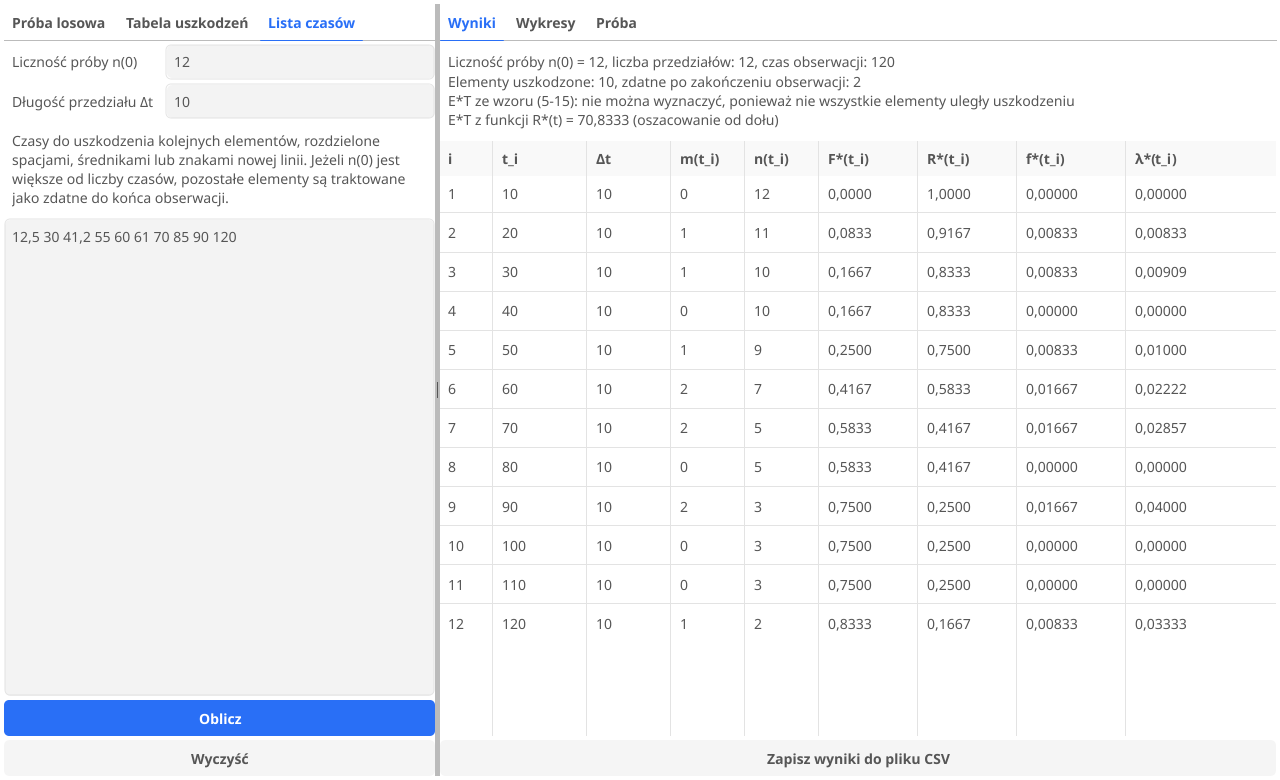
\includegraphics[width=\textwidth]{08_times_results}
  \caption{Wyniki dla listy czasów przy niepełnej próbie}
  \label{fig:times}
\end{figure}

Wyniki sprawdzono rachunkiem ręcznym. Przykładowo do przedziału $(50, 60]$ należą
czasy 55 i~60 (czas leżący na granicy trafia do niższego przedziału), a~na jego
początku zdatnych jest 9~elementów, zatem
\begin{equation*}
  F^*(60) = \frac{5}{12} = 0{,}4167, \qquad
  f^*(60) = \frac{2}{12 \cdot 10} = 0{,}01667, \qquad
  \lambda^*(60) = \frac{2}{9 \cdot 10} = 0{,}02222,
\end{equation*}
co zgadza się z~szóstym wierszem tabeli. Dwa elementy pozostały zdatne, więc
$R^*(120) = 2/12 = 0{,}1667$. Program poprawnie informuje, że $E^*T$ ze wzoru (5-15)
nie da się wyznaczyć, i~podaje oszacowanie od dołu $70{,}83$ z~całkowania $R^*(t)$.

\subsection{Obsługa błędnych danych}

Program nie wykonuje obliczeń dla błędnych danych, tylko wyświetla okno z~opisem
błędu (rys.~\ref{fig:error}), a~poprzednie wyniki pozostają bez zmian. Sprawdzone
przypadki zestawiono w~tab.~\ref{tab:errors}.

\begin{table}[H]
  \centering
  \caption{Reakcja programu na błędne dane}
  \label{tab:errors}
  \small
  \begin{tabular}{@{}p{0.36\textwidth}p{0.6\textwidth}@{}}
    \toprule
    Wprowadzone dane & Komunikat \\
    \midrule
    pusta tabela uszkodzeń & tabela uszkodzeń jest pusta \\
    $n(0)$ = ,,abc'' & Liczność próby n(0): ,,abc'' nie jest poprawną liczbą całkowitą \\
    tabela z~przykładu 5.1 przy $n(0) = 10$ & pozycja 4: łączna liczba uszkodzeń przekracza
      liczność próby n(0) \\
    wiersz tabeli z~jedną wartością & wiersz 2: oczekiwano dwóch wartości: t oraz m(t) \\
    parametr $\lambda = -1$ & parametr $\lambda$ musi być dodatni \\
    ziarno generatora ,,x'' & Ziarno generatora: ,,x'' nie jest nieujemną liczbą całkowitą \\
    liczność próby losowej $n = 0$ & liczność próby musi być liczbą dodatnią \\
    $\Delta t = 0$ & długość przedziału $\Delta t$ musi być dodatnia \\
    lista czasów ,,1 x 3'' & pozycja 2: ,,x'' nie jest poprawną liczbą \\
    trzy czasy przy $n(0) = 2$ & liczność próby n(0) jest mniejsza od liczby podanych czasów \\
    \bottomrule
  \end{tabular}
\end{table}

\begin{figure}[H]
  \centering
  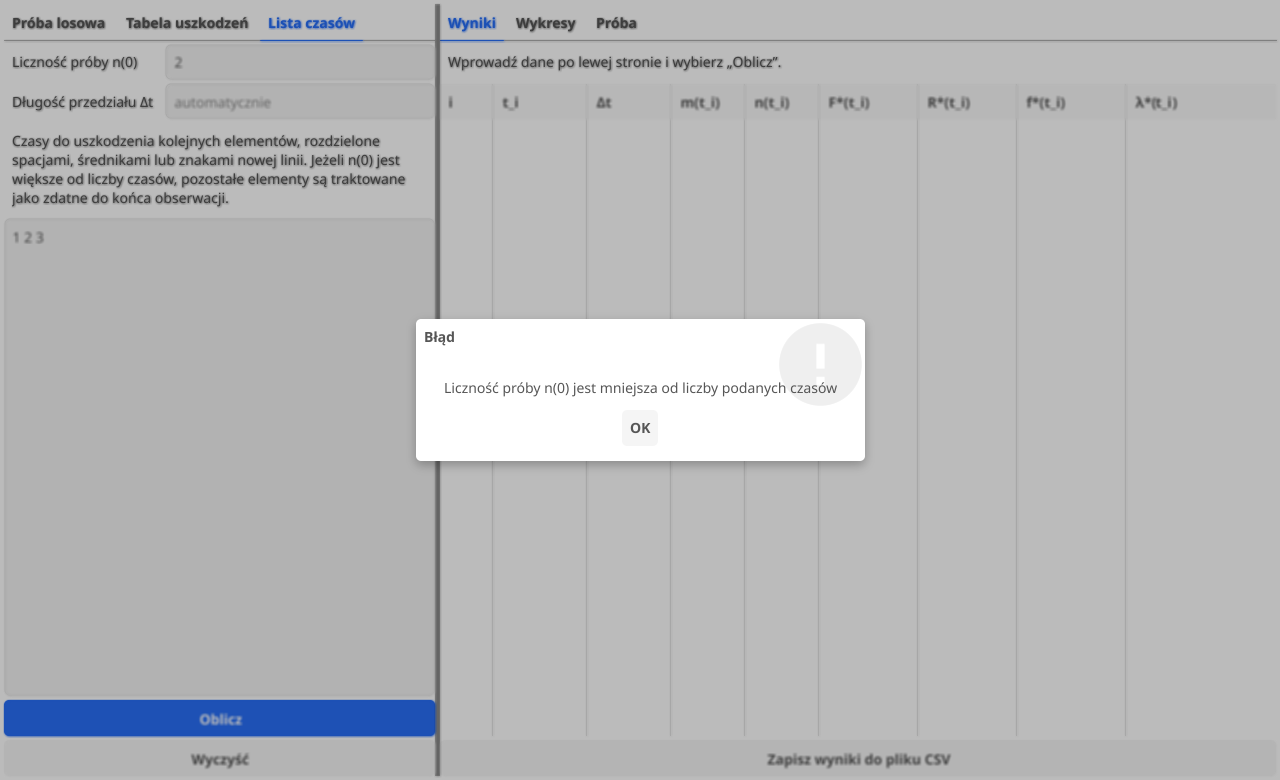
\includegraphics[width=0.78\textwidth]{09_error_dialog}
  \caption{Komunikat o~błędnych danych}
  \label{fig:error}
\end{figure}

\subsection{Wnioski}

\begin{itemize}
  \item Program odtwarza wyniki przykładów 5.1--5.4 z~książki z~dokładnością do
    zaokrągleń w~niej zastosowanych.
  \item Dla prób losowych wskaźniki empiryczne zbliżają się do teoretycznych wraz ze
    wzrostem liczności próby, zgodnie z~oczekiwaniami.
  \item Empiryczna intensywność uszkodzeń wyznaczana ze wzoru (5-12) jest zaniżona
    tym bardziej, im dłuższy jest przedział $\Delta t$; długość przedziału trzeba
    więc dobierać jako kompromis między tym błędem a~rozrzutem wyników.
  \item Błędne dane są wykrywane przed obliczeniami i~opisywane komunikatem
    wskazującym miejsce błędu.
\end{itemize}
